\documentclass[lettersize,journal]{IEEEtran}

\usepackage[utf8]{inputenc}
\usepackage{lmodern}
\usepackage[T1]{fontenc}
\usepackage{mathtools}
\usepackage{float}
\usepackage{csvsimple}
\providecommand{\abs}[1]{\lvert#1\rvert}
\usepackage{braket}
\providecommand{\eq}[2]{
    \begin{equation}
        #2
    \label{eq:#1}
    \end{equation}
}
\providecommand{\eqgat}[2]{
    \begin{gather}
        #2
    \label{eq:#1}
    \end{gather}
}
\usepackage{amsmath}
\DeclareMathOperator{\calA}{\mathcal{A}}
\DeclareMathOperator{\calB}{\mathcal{B}}
\DeclareMathOperator{\calH}{\mathcal{H}}
\DeclareMathOperator{\tr}{tr}
\usepackage{fancyhdr}
\usepackage{authblk}
\usepackage{abstract}
\usepackage{wrapfig}
\usepackage{graphicx}
\usepackage{hyperref}

\usepackage[backend=biber,style=phys]{biblatex}
\addbibresource{TFG.bib}

% \usepackage{multirow}
% \usepackage[table,xcdraw]{xcolor}

% \usepackage{graphicx}
% \usepackage{caption}
% \usepackage{subcaption}

% \usepackage[a4paper]{geometry}
% \geometry{top=3cm, bottom=3.3cm, left=3cm, right=3cm}


\title{Entanglement Entropy and Holography}
\author{Ferran Rodríguez Mascaró}
\date{}


\begin{document}


\twocolumn[
    \begin{@twocolumnfalse}
        \maketitle{}
        \begin{abstract}
            The AdS/CFT correspondance, also called Holography, is a duality relating quantum field theory and gravity, in particular conformal field theory and anti-de Sitter spacetime-time gravities. It descrives how quantities from each of these theories, the so-called holographic dictionary, can be studied one throw the other. One of the most important magnituds of the holographic dictionary is the entanglement entropy of a region, that mesures the degree of quantum entanglement between this region and its surroundings. In this work it is introduced the basics of holography, especially aplied to entanglement entropy, demonstrating some important properties and fascinating achievements of the theory, as the equivalence of the Ryu-Takayanagi formula with the Bekenstein-Hawking black hole entropy formula, the fulfillment of the strong subadditivity property or the duality between entanglement entropy and the Einstein field equations.
        \end{abstract}
    \end{@twocolumnfalse}
]


\section{Introduction} \label{s:Intro}

---

---

---



\subsection{Anti-de Sitter space-times} \label{ss:AdS}

An anti-de Sitter (AdS) space-time is a maximally symmetric spacetime with negative curvature, solution to Einstein field equations with a negative cosmological constant.

% A maximally symmetric spacetime with negative curvature, solution to Einstein's equations with a negative cosmological constant, is called an anti-de Sitter (AdS) spacetime.

% Its Riemann tensor is expressed as
% \begin{equation}
%     R_{abcd} = - \frac{1}{L^2} ( g_{ac} g_{bd} - g_{ad} g_{bc} ) ,
% \label{eq:AdS_Riemann}
% \end{equation}
% One can find that for these type of space-times to be solution of Einstein equations, the cosmological constant must be
% \begin{equation}
%     \Lambda = - \frac{(D-1)(D-2)}{2L^2} .
% \label{eq:AdS_cosmo-const}
% \end{equation}

One can obtain the metric of the half-space of an AdS spacetime of $D=d+1$ dimensions using the coordinate system of the Pointcaré patch as
\eq{AdS_PP-metric}{
    ds_{AdS_D}^2 = \frac{1}{z^2} \left( -dt^2 + dz^2 + \sum_{i=1}^{d-1} dx_i^2 \right) \ ,
}
with the time and space-related dimensions $t , x_i \in (-\infty,+\infty)$ and an extra dimension $z \in (0,+\infty)$ \cite{kaplan_lectures_nodate}.

Fixing the coordinate $z$, one creates $d$-dimensional space-time surfaces 'weighted' by the factor $\frac{1}{z^2}$.

\begin{wrapfigure}{r}{0.27\textwidth}
    \centering
    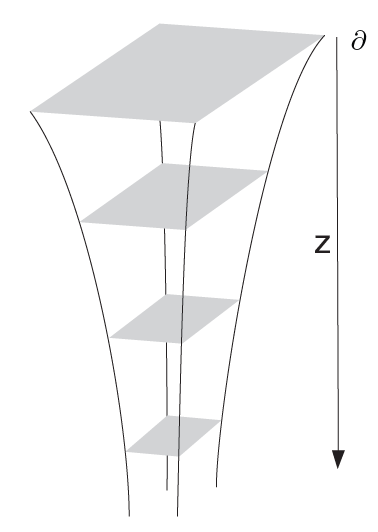
\includegraphics[width=0.15\textwidth]{../Imatges/Extern/Captura_Superficies_z.png}
\caption{Representation of the different Minkowski space-time layers along the $z$ coordinate inside an AdS space-time.}
\label{fig:AdS_z-surfaces}
\end{wrapfigure}

At constant time, \cite{} this metric forms hyperbolic spaces of negative curvature, conformally equivalent to Minkowski space-times at $z \to 0$. The conformal infinity of AdS is timelike, thus one needs boundary conditions to determine the future evolution uniquely.
% \footnotetext{A conformal or angle-preserving function is the one that preserves angles between curves at a certain point, as well as preserving orientation \cite{}.}

Using hyper-polar coordinates one can obtain a different expression for the metric which covers the entire space:
\eq{AdS_hyper-polar-metric}{
    ds_{AdS_D}^2 = \left [ - \left ( 1 + \frac{r^2}{L^2} \right ) dt^2 + \frac{dr^2}{\left ( 1+ \frac{r^2}{L^2} \right )} + r^2 d \Omega_{D-2}^2 \right ] \ ,
}
being $L$ ($k^2=1/L^2$) the so-called anti-de Sitter radius.

\begin{wrapfigure}{r}{0.27\textwidth}
    \centering
    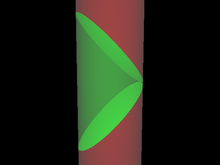
\includegraphics[width=0.21\textwidth]{../Imatges/Extern/Wikipedia_Half-space_Cilindric.png}
\caption{Representation of the half-space region of an AdS space-time and its boundary.}
\label{fig:AdS_cylindrical}
\end{wrapfigure}

In figure \ref{fig:AdS_cylindrical} it is represented the metric of equation \ref{eq:AdS_hyper-polar-metric}. The whole cylinder corresponds to an AdS space-time, being the lateral surface the conformal boundary (where $z \to 0$, or $r \to \infty$). The marked region corresponds to the one covered by the half-space coordinates, flanked by the conformal boundary and two lightlike geodesic hyperplanes \cite{}.


\subsection{Conformal Field Theories} \label{ss:CFT}

A conformal field theory (CFT) is a quantum field theory that is invariant under transformations that locally preserve angles.


\subsection{The Holographic Principle} \label{ss:Holography}

The covariant entropy bound \cite{bousso_covariant_1999} is conjectured as the representation of the universal law, in a four-dimensional space-time on which Einstein’s equation is satisfied, in which the entropy of a system is bounded by its area. It says that the number of independent degrees of freedom on any light-sheet of a surface cannot exceed a quarter of the area of this surfaces.

This bound implies that the degrees of freedom inside some region grows with the area of the boundary and not as the volume of the region. This behavior leads to the \textit{holographic principle}, wich states that in a quantum gravity theory all the physics phenomena within some volume can be described in terms of a theory on the boundary of the area of the volume, which has less than one degree of freedom per Planck area \cite{t_hooft_dimensional_2009}.


\subsection{AdS/CFT Correspondance} \label{ss:AdS/CFT}

A class of conformal field theories are equivalently described in certain limits in terms of anti-de Sitter space-times \cite{rangamani_holographic_2017}.

The \textit{AdS/CFT Correspondance}, simply called \textit{holography} or \textit{gauge/gravity correspondance} \cite{ramallo_introduction_2013}, is an equivalence or duality between quantum gravity theories (certain string theories) at asymptotically $D$-dimensional anti-de Sitter space-times and non-gravitational conformal quantum field theories at Minkowski space-times of $D-1$ dimensions \cite{maldacena_large_1999}. It allows us to study different aspects of each of these theories through the other. The so-called \textit{holographic dictionary} relates quantities (observables) between the AdS theories and the CFT. % \cite{kaplan_lectures_nodate}


\section{Entanglement Entropy} \label{s:EE}

When two quantum systems enter into temporary physical interaction, they can no longer be described in the same way after a time of mutual influence \cite{schrodinger_discussion_1935}. One can no longer describe neither of those systems independently without losing global information, because the state of each systems know is influenced and correlated by the other system. This is the so-called \textit{quantum entanglement}.

Being two quantum systems represented by the corresponding Hillberg spaces $\calH_A$ and $\calH_B$, and an state $\ket{\Psi} \in \calH = \calH_A \otimes \calH_B$, this would be an entangled state if
\eq{entanglement}{
    \ket{\Psi} \neq \ket{\Psi_A} \otimes \ket{\Psi_B} \ \longrightarrow \ \ket{\Psi} = \sum_{i,j} c_{ij} \ket{i}_A \otimes \ket{j}_B \ ,
}
being $\ket{\Psi_{A,B}}$ the possible different substates in which one could separate $\ket{\Psi}$ if it was separable, substates expressed in each orthonormal bases $\{ \ket{k}_{A,B} \}$ of $\calH_{A,B}$ \cite{}.

The \textit{entanglement entropy} is a measure of the degree of quantum entanglement between the two subsystems composing a full quantum system \cite{nishioka_entanglement_2018}. It is defined by the von
Neumann entropy of the reduced density matrix $\rho_A$ of one of the subsystems as
\eq{EE}{
    S_{EE}(A) = - \tr_A ( \rho_A \log \rho_A ) \ ,
}
being $\rho_A = \tr_B \ket{\Psi}\bra{\Psi}$. If $\rho_A$ is diagonalized ($\rho_A = \sum_i \lambda_i \ket{i}\bra{i}$), then the entanglement entropy would take the simplified form $S_{EE} = - \sum_i \lambda_i \log \lambda_i$.

If there is no entanglement between both subsystems, the entanglement entropy is null ($S_{EE} = 0$).


\subsection{Entanglement entropy in CFT} \label{ss:EE_CFT}

The general expression of the entanglement entropy for a $d$-dimensional quantum field theory is

\eqgat{EE}{
    S_{QFT_d} = c_{d-2} \left( \frac{H}{\delta} \right) ^{d-2} + c_{d-1} \left( \frac{H}{\delta} \right) ^{d-4} + ... + \nonumber \\
    + \begin{dcases}
        c_1 \frac{H}{\delta} + (-1)^{\frac{d-1}{2}} s_{\text{non-loc}}
        \qquad \qquad \qquad \quad \ \text{for odd } d \\
        c_2 \left ( \frac{H}{\delta} \right ) + (-1)^{\frac{d-2}{2}} s_{\text{loc}} \log \left ( \frac{H}{\delta} \right ) + c_0
        \quad \text{for even } d
    \end{dcases} \ ,
}
% \begin{equation*}
%     S_{QFT_d} = c_{d-2} \left( \frac{H}{\delta} \right) ^{d-2} + c_{d-1} \left( \frac{H}{\delta} \right) ^{d-4} + ... +
% \end{equation*}
% \eq{EE}{
%     +
%     \begin{dcases}
%         c_1 \frac{H}{\delta} + (-1)^{\frac{d-1}{2}} s_{\text{non-loc}}
%         & \text{for odd } d \\
%         c_2 \left ( \frac{H}{\delta} \right ) + (-1)^{\frac{d-2}{2}} s_{\text{loc}} \log \left ( \frac{H}{\delta} \right ) + c_0
%         & \text{for even } d
%     \end{dcases} \ ,
% }
% \eq{EE}{
%     \begin{array}{cc}
%         {S_{QFT_d} = c_{d-2} \left( \frac{H}{\delta} \right) ^{d-2} + c_{d-1} \left( \frac{H}{\delta} \right) ^{d-4} + ... + } \\ \\
%         {+ \left \{ \begin{array}{cl} 
%         c_1 \frac{H}{\delta} + (-1)^{\frac{d-1}{2}} s_{\text{non-loc}}
%         & \text{for odd } d \\
%         c_2 \left ( \frac{H}{\delta} \right ) + (-1)^{\frac{d-2}{2}} s_{\text{loc}} \log \left ( \frac{H}{\delta} \right ) + c_0
%         & \text{for even } d
%         \end{array} \right . \ ,}
%     \end{array}
% }
\cite{nishioka_entanglement_2018} in which $H$ is the characteristic length of the region studied, $c_i$ are coefficients that are non-universal (not well-defined in the continuum, dependent on the definition of $\delta$) and local, and $s_{\text{loc},\text{non-loc}}$ are universal coefficients (the suffixs refer to if they are local or non-local) that contain information about the corresponding CFT.


\subsection{Entanglement entropy in AdS/CFT} \label{ss:EE_AdS/CFT}

\begin{wrapfigure}{r}{0.27\textwidth}
    \centering
    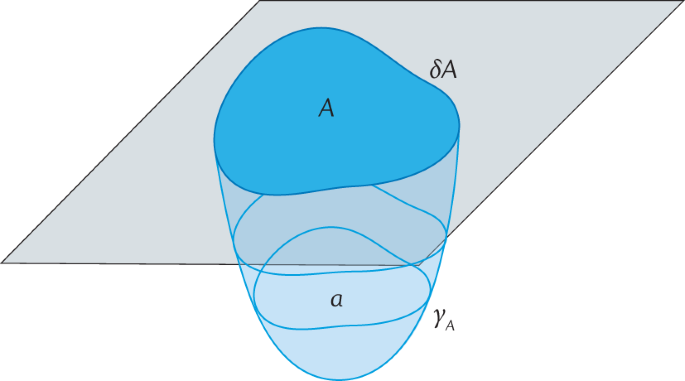
\includegraphics[width=0.27\textwidth]{../Imatges/Extern/EE_AdS-CFT.png}
\caption{Region $\calA$ (dark blue) and its boundary $\partial \calA$ inside a $z=\delta$ AdS slide (grey) and its respective $\gamma_{\calA}$ (light blue) inside the AdS space-time.}
\label{fig:EE_AdS-CFT}
\end{wrapfigure}

In a quantum field placed in a Minkowski space-time, at a given time, every point on space is entangled with the points surrounding it \cite{nishioka_entanglement_2018}. Therefore, the entanglement entropy between a subsytem and the rest of the space will be dominated by the correlations between both sides of the boundary that isolates the subsystem.

% \begin{wrapfigure}{r}{0.25\textwidth}
%     \centering
%     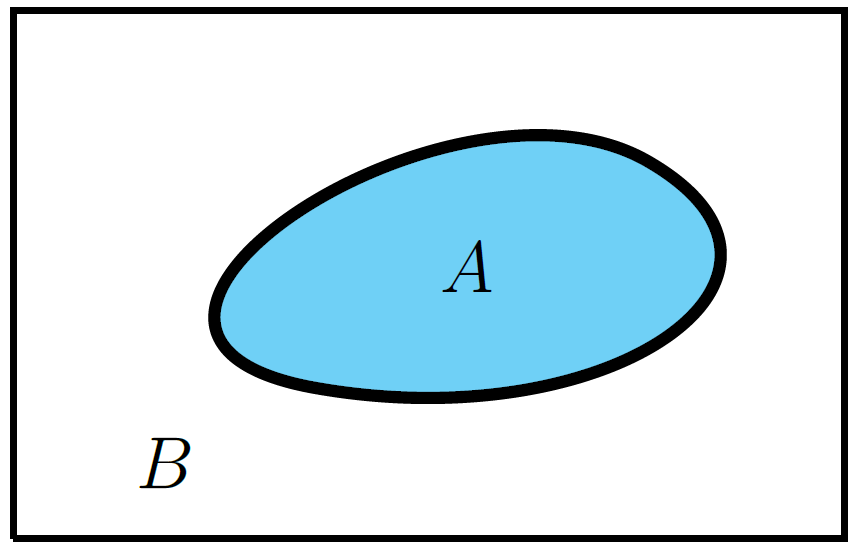
\includegraphics[width=0.24\textwidth]{../Imatges/Captura_EE_Frontera.png}
% \caption{Bipartion of a system in two complementary regions A and B.}
% \label{fig:EE_Minkowski-boundary}
% \end{wrapfigure}

% \begin{figure}[h!]
%     \centering
%     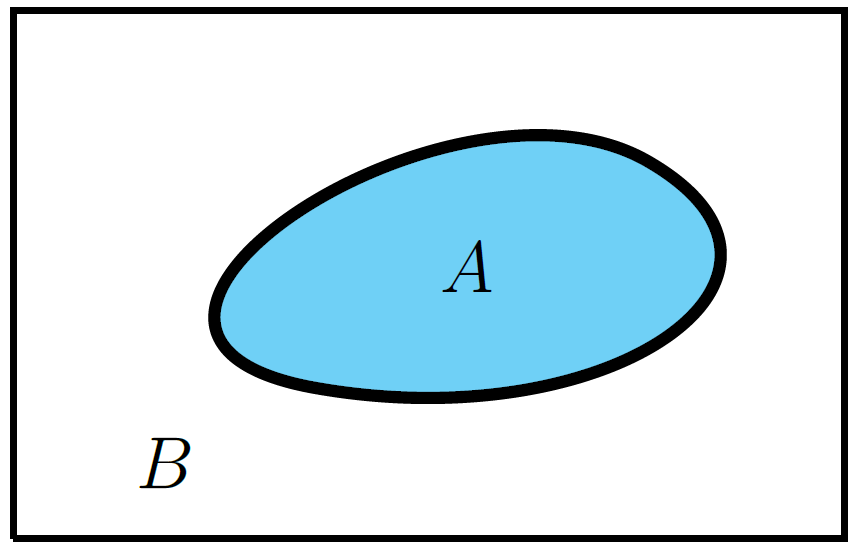
\includegraphics[scale=0.2]{../Imatges/Captura_EE_Frontera.png}
% \caption{Bipartion of a system in two complementary regions A and B.}
% \label{fig:EE_Minkowski-boundary}
% \end{figure}

In an ($d+1$)-dimensional AdS space-time, being $\calA$ a region of a $d$-dimensional Minkowski space-time slice formed from fixing $z$ as $z=\delta \ll 1$, the entanglement entropy of a $d$-dimensional CFT on this Minkowski space-time will be expressed by the so-called Ryu-Takayanagi formula
\eq{EE_RT}{
    S_{\calA} = \frac{ \text{Area}(\gamma_{\calA}) }{ 4 G_{d+1} } \ ,
}
\cite{ryu_holographic_2008} where $\gamma_{\calA}$ is the surface of minimal area on the whole AdS space-time connected to the ($d-1$)-dimensional boundary $\partial \calA$ of the region $\calA$, and $G_{d+1}$ is the ($d+1$)-dimensional Newton constant (represented in figure \ref{fig:EE_AdS-CFT}).

The area of $\gamma_{\calA}$ is obtained by
\eq{EE_RT-area}{
    \text{Area}(\gamma_{\calA}) = \int_{\gamma_{\calA}} \sqrt{h} \ d^{d}y \ ,
}
where $y$ are the $d$ coordinates that represent surface $\gamma_{\calA}$ and $h$ is the determinant of the metric $h_{ij} = \frac{\partial x^\mu}{\partial y^i} \frac{\partial x^\nu}{\partial y^j} g_{\mu\nu}$ induced on the surface by the surrounding space-time.

The Ryu-Takayanagi formula is valid for generic systems, and gives a flavour of how the geometry of space-time can emerge from mere quantum information. As a curiosity, the Ryu-Takayanagi formula in the case of a thermalized system of particles in an AdS space-time derives to the Bekenstein-Hawking formula \cite{bekenstein_black_1973} for the entropy a black hole:
\eq{BH}{
    S_{BH} = \frac{ A_H }{ 4 G } \ ,
}
that says that the entropy related to a black hole only depends on the area $A_H$ of its event horizon.

From the Ryu-Takayanagi formula for a ( $d+1$ )-dimensional anti-de Sitter space-time one obtains the expected general expression of the entanglement entropy \ref{eq:EE} for a $d$-dimensional conformal field theory \cite{}.

To do so, one defines the region studied $\calA$ of a layer with $z = \delta \ll 1$ in terms of an apropiate group of coordinates $x_i$. The surface of minimal area $\delta_{\calA}$ will be defined in terms of these set of coordinates, being $z = f (x_i)$. Aplying this restriction to the metric one obtains the induced metric onto $\delta_{\calA}$. The square rood of the determinant of the induced metric, $\sqrt{h}$, is integrated to obtain the family of surface of $\delta_{\calA}$. Extremezing this functional one obtains the surface of minimal area $\delta_{\calA}$. The induced metric will be expressed in terms of $f(x_i)$ and its derivate, so one can use the equations of Euler-Lagrange to find relations between $f (x_i)$ and its derivate to finally deduce its expression and solve the integral.


\section{Strong subadditivity} \label{s:SS}

Being $S(\rho)$ the von Neumann entropy (Equation \ref{eq:EE}) of a system with density matrix $\rho$, two entanglement subsystems $\rho_1$ and $\rho_2$ forming a whole system with $\rho_{full}$ generally obey the inequalities
\eq{EE_subadd}{
    \abs{S(\rho_1)-S(\rho_2)} \le S(\rho_{full}) \le S(\rho_1) + S(\rho_2) \ .
}
This property of the entanglement entropy is known as \textit{subadditivity} \cite{headrick_holographic_2007}.

These relations between entanglement entropies of the different subsystems can be extended to a higer number of subsystems. For example, in the case of three subsystems we have that
\eqgat{EE_strong-subadd}{
    S(\rho_{12}) + S(\rho_{23}) \ge S(\rho_2) + S(\rho_{123}) \ , \nonumber \\
    S(\rho_{12}) + S(\rho_{23}) \ge S(\rho_1) + S(\rho_3) \ ,
}
or equivalently
\eqgat{EE_strong-subadd-2}{
    S(\rho_{A}) + S(\rho_{B}) \ge S(A \cup B) + S(A \cap B) \ , \nonumber \\
    S(\rho_{A}) + S(\rho_{B}) \ge S(A \setminus B) + S(B \setminus A) \ .
}
This is called \textit{strong subadditivity}.

\begin{wrapfigure}{r}{0.2\textwidth}
    \centering
    
\includegraphics[width=0.2\textwidth]{../Imatges/empty.png}
\caption{}
\label{fig:}
\end{wrapfigure}

An important test of the validity of the Ryu-Takayanagi formula (Equation \ref{eq:EE_RT}) is whether it has the property of strong subadditivity, that should be fulfilled in any quantum mechanical theory.

Generally, this property is very difficult to demonstrate, but is extremely easy to do so using the Ryu-Takayanagi formula only using geometric relations.

Let's start proving the first inequality. Let $\gamma_{\calA}$, $\gamma_{\calB}$ be the surfaces of minimal area in the bulk connected to $\partial \calA$, $\partial \calB$ respectively, and $r_{\calA}$, $r_{\calB}$ the corresponding regions of the bulk. Thus, $\partial r_{\calA} = \calA \cup \gamma_{\calA}$, $\partial r_{\calB} = \calB \cup \gamma_{\calB}$, and we define the regions
\eq{SS_r-1}{
    r_{\calA \cup \calB} = r_{\calA} \cup r_{\calB} \ , \ r_{\calA \cap \calB} = r_{\calA} \cap r_{\calB} \ .
}
The surfaces onto the slice of this regions can be decomposed as
\eq{SS_dr-1}{
    \partial r_{\calA \cup \calB} = (\calA \cup \calB) \cup \gamma_{\calA \cup \calB} \ , \ \partial r_{\calA \cap \calB } = (\calA \cap \calB) \cup \gamma_{\calA \cap \calB} \ .
    }
It is clear that $\partial (\calA \cup \calB)$ and $\partial (\calA \cap \calB)$ correspond to $\gamma_{\calA \cup \calB}$ and $\gamma_{\calA \cap \calB}$, but nothing says that they are the surfaces of minimal area $\gamma^{\text{min}}_{\calA \cup \calB}$ and $\gamma^{\text{min}}_{\calA \cap \calB}$ related to $\partial (\calA \cup \calB)$ and $\partial (\calA \cap \calB)$, they are upper bounds. This proves that
\eq{SS_gamma-1}{
    \gamma_{\calA} + \gamma_{\calB} = \gamma_{\calA \cup \calB} + \gamma_{\calA \cap \calB} \ge \gamma^{\text{min}}_{\calA \cup \calB} + \gamma^{\text{min}}_{\calA \cap \calB} \ ,
}
and, therefore, using the Ryu-Takayanagi formula (Equation \ref{eq:EE_RT}), the first inequality of equation \ref{eq:EE_strong-subadd-2}.

Regarding the second inequality, we see that
\eq{SS_r-2}{
    r_{\calA \setminus \calB} = r_{\calA} \cup r_{\calB} \ , \ r_{\calB \setminus \calA} = r_{\calB} \cup r_{\calA} \ .
}
The surface onto the slice of this regions are decomposed as
\eq{SS_dr-2}{
    \partial r_{\calA \setminus \calB} = (\calA \setminus \calB) \cup \gamma_{\calA \setminus \calB} \ , \ \partial r_{\calB \setminus \calA } = (\calB \setminus \calA) \cup \gamma_{\calB \setminus \calA} \ .
}
The $\partial (\calA \setminus \calB)$ and $\partial (\calB \setminus \calA)$ correspond to the upper bounds $\gamma_{\calA \setminus \calB}$ and $\gamma_{\calB \setminus \calA}$ of the surfaces of minimal area $\gamma^{\text{min}}_{\calA \setminus \calB}$ and $\gamma^{\text{min}}_{\calA \setminus \calB}$. So
\eq{SS_gamma-2}{
    \gamma_{\calA} + \gamma_{\calB} = \gamma_{\calA \setminus \calB} + \gamma_{\calB \setminus \calA} \ge \gamma^{\text{min}}_{\calA \setminus \calB} + \gamma^{\text{min}}_{\calB \setminus \calA} \ ,
}
and, through the Ryu-Takayanagi formula, the second inequality of \ref{eq:EE_strong-subadd-2} it is proven.

Using this simple geometric proof, it is shown that holography presents the strong subadditivity property that should be true in any quantum mechanical many-body system, playing the extra dimension in the holographic dual an essential role.

In the holographic context, the only examples where these inequalities saturate involve only two disjoint regions, and therefore reduce to the saturation of weak subadditivity.

The first inequality of equation \ref{eq:EE_subadd}, called Araki-Lieb inequality, is saturated when the full system is pure, and the entanglement entropy of each subsystem are due only to correlations between each other and not because the full system is in a mixed state.

Another case where this inequality is saturated is when there is a black hole inside the bulk, $\calA$ corresponds to a region outside the black hole and $\calB$ includes two connected components: $\calA$ and the event horizont, being $\partial \calA = \partial \calB$. In this case, $S(\calB) = S(\calA) + S_{BH}$, where $S_{BH}$ is the black hole's Bekenstein-Hawking entropy. Since due to the limit of the information that the bulk can contain $S_{full} = S_{BH}$, the Araki-Lieb inequality is saturated.

The second inequality is saturated when the mutual information
\eq{Mutual-Info}{
    I(\calA,\calB) = S(\calA) + S(\calB) - S(\calA \cup \calB)
}
is zero. In this case, the two regions are sufficiently far apart that their union's surface is simply the union of their minimal surfaces. The mutual information only vanishes when the two subsystems are uncorrelated. It is interesting that the correlations between subsystems can go stricktly to zero in a field theory in the limit of large number of subsystems.


\section{Entanglement entropy for higher orders} \label{s:EE_HO}

It has been shown that the Ryu-takayanagi formula (\ref{eq:EE_RT}) as the entanglement entropy for holographic theories dual to Einstein gravity. Nevertheless, working with effective actions makes higher-order terms appear as stringy and quantum corrections \cite{bueno_holographic_2021}.


\subsection{Higher curvatures} \label{ss:StringyC}

For higher-curvature gravities (or stringy corrections), the area functional needs to be modified, similarly to the way the Bekenstein-Hawking formula for the entropy of a black hole (\ref{eq:BH}) is replaced by Wald formula \cite{iyer_properties_1994}. But replacing the functional of the entanglement entropy for the Wald's one does not work \cite{bueno_holographic_2021}. Additional "anomaly" terms corresponding to extrinsic curvatures of the generalized surface involving arbitrary contractions of Riemann tensors and metrics are required \cite{dong_holographic_2014}. Schematically:
\eq{EE_HO}{
    S_{\text{HO}}(\calA) = S_{\text{Wald}} + S_{\text{Anomaly}} \ .
}

In the same way that one finds the entanglement entropy with the Ryu-Takayanagi formula (expained in Section \ref{ss:EE_AdS/CFT}), the generalized holographic surface should be obtained by extremizing the new functional with the corrections of the previous expression. In the anomaly term, each of the Riemann tensor components resulting has to be split into summatories of different weighted terms. The way that this terms are weighted is nonunique, leading to the so-called \textit{splitting problem}.


\subsection{Quantum corrections} \label{ss:QuantumC}

One can also consider corrections on the Ryu-Takayanagi formula realted to quantum mechanical effects in the bulk \cite{faulkner_quantum_2013}.

This quantum corrections are essentially given by the entanglement entropy between the bulk bounded by the minimal area surface and the outside region. One can see the bulk region as an effective field theory itself living on a fixed background geometry and compute its entanglement entropy as in any quantum field.

One has to be cautious and do not confuse this entanglement entropy with the one computed by the Ryu-Takayanagi formula which is intended to be generalized.








\section{Duality with Einstein field equations} \label{s:EQ}

\subsection{First law of entanglement entropy} \label{ss:FLEE}

For a small perturbation of a quantum field theory state $\ket{\psi(\varepsilon)}$ to the initial state $\ket{\psi(0)}$, the \textit{First Law of Entanglement Entropy} is defined as
\eq{FLEE}{
    \delta S_{\calA} = \frac{d}{d \varepsilon} S_{\calA} = \frac{d}{d \varepsilon} \abs{H_{\calA}} = \frac{d}{d \varepsilon} \tr (H_{\calA} \rho_{\calA}) \equiv \delta E_{calA}
}
for the entanglement entropy of a subsystem $\calA$ \cite{fareghbal_first_2019}. The modular Hamiltonian $H_{\calA}$ is independent of the perturbaton and is defined by
\eq{modularH}{
    \rho_{\calA} (\varepsilon) = e^{-H_{\calA}}.
}

The first law of entanglement entropy is a generalization of the first law of thermodynamics for any arbitrary small perturbation, quantum state or subsystem.

When $H_{\calA}$ is a local operator, $\rho_{\calA}$ can be mapped to a thermal one, $\rho_{\calH}$, by an unitary transformation, being the resultant entropy thermal. Hence $\rho_{\calH}$ can be written as
\eq{modularH2}{
    \rho_{\calH} = \frac{e^{-H_{\calH}}}{\tr (e^{-H_{\calH}})} \ ,
}
where $H_{\calH}$ is the associated charge of the so-called modular flow $\xi$.

In the holographic description \cite{fareghbal_first_2019} it has been shown that writing both sites of the first law of entanglement entropy in terms of the corresponding bulk parameters leads to a constraint on the bulk geometry that is exactly the Einstein field equations. If this was an intrinsec property of any gauge/gravity theory, one could use entanglement entropy in an arbitrary field theory to find a dual gravitational geometry.

\subsection{First law of entanglement entropy applied to holography} \label{ss:FLEE_H}

---

---

---




\section{Conclusions} \label{s:Conclusions}

---

---

---




\section{Acknoledgments} \label{s:Acknoledgments}

---

---

---




\printbibliography

\end{document}